\documentclass{article}
\usepackage[utf8]{inputenc}

\usepackage{tikz}
\usetikzlibrary{positioning}

\begin{document}

% %------------------------------------------------------------------------------
% %Introductory example
% \begin{figure}[p]
% \begin{tikzpicture}
% \filldraw[black] (0,0) circle (2pt) node[anchor=west] {Intersection point};
% %\draw[gray, thick] (-1,2) -- (2,-4); % longer diagonal
% %\draw[gray, thick] (-1,-1) -- (2,1); % shorter diagonal

% \draw[gray, thick] (-1,2) -- (-1,-1); % left border
% \draw[gray, thick] (2,1) -- (2,-4);   % right border
% \draw[gray, thick] (-1,2) -- (2,1);   % top border
% \draw[gray, thick] (-1,-1) -- (2,-4);   % bottom border
% \end{tikzpicture}
% \end{figure}
% %------------------------------------------------------------------------------


%------------------------------------------------------------------------------
%Introductory example
\setcounter{figure}{1}
\begin{figure}[p]
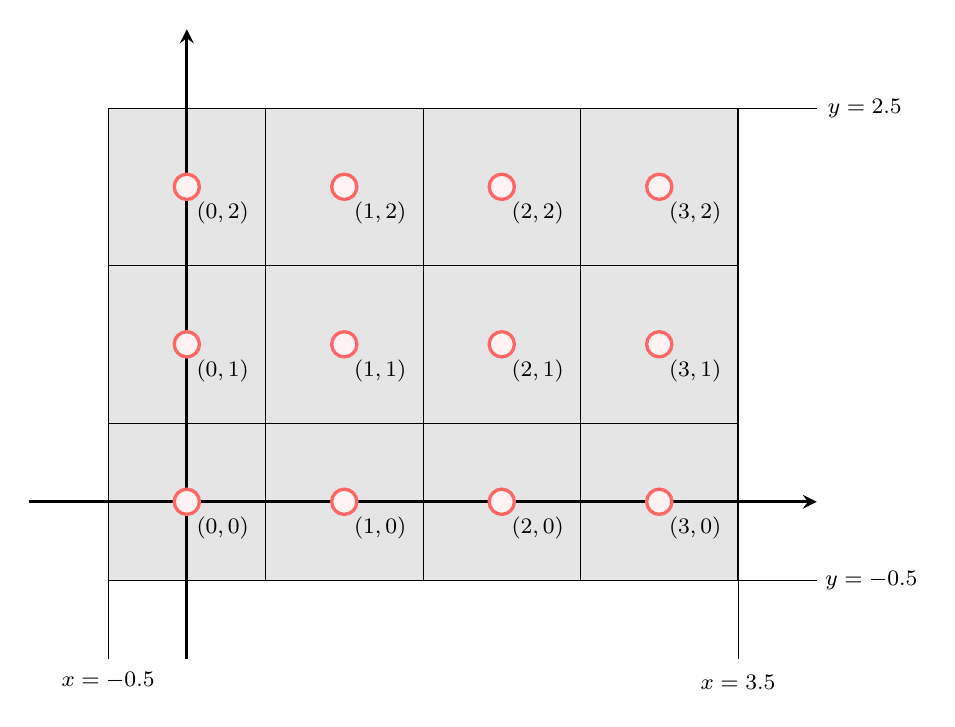
\begin{tikzpicture}[>=stealth, scale=2]
  % definition of a basic style.
  \tikzstyle help lines=[color=black,very thin]
  % The background rectangle that works as a filling in rectangle
  \filldraw[fill=gray!20!white, step=1,  xshift=-0.5cm, yshift=-0.5cm]
    (0cm,0cm) rectangle (4cm,3cm);
  % The grid
  \draw[step=1, style=help lines, xshift=-0.5cm, yshift=-0.5cm]
    (0cm,0cm) grid (4cm,3cm);

  % The coordinate axes.
  \draw[->, very thick] (-1.,0) -- (4,0); % X axis
  \draw[->, very thick] (0,-1.) -- (0,3); % Y axis
  
  % support vertical, horizontal lines.
  \draw[very thin] (3.5,2.5) -- (4,2.5) node[xshift=1.2cm,anchor=east] {\footnotesize$y=2.5$};
  \draw[very thin] (3.5,-0.5) node{} -- (4,-0.5) node[xshift=1.4cm,anchor=east] {\footnotesize$y=-0.5$};
  \draw[very thin] (3.5,-0.5) -- (3.5,-1.) node[yshift=-0.5cm,anchor=south] {\footnotesize$x=3.5$};
  \draw[very thin] (-0.5,-0.5) -- (-0.5,-1.) node[yshift=-0.5cm,anchor=south] {\footnotesize$x=-0.5$};

  % Row of circles
  \foreach \x in {0,...,3}
        \filldraw [color=red!60, fill=red!5, very thick] (\x,0) circle (0.08cm);
  \foreach \x in {0,...,3}
        \filldraw [color=red!60, fill=red!5, very thick] (\x,1) circle (0.08cm);
  \foreach \x in {0,...,3}
        \filldraw [color=red!60, fill=red!5, very thick] (\x,2) circle (0.08cm);
  % Coordinates
  \foreach \x in {0,...,3}
    \draw (\x cm,-0.3cm) node[anchor=south west] {\footnotesize$(\x, 0)$};
  \foreach \x in {0,...,3}
    \draw (\x cm,0.7cm) node[anchor=south west] {\footnotesize$(\x, 1)$};
  \foreach \x in {0,...,3}
    \draw (\x cm,1.7cm) node[anchor=south west] {\footnotesize$(\x, 2)$};
    
  %  \filldraw[color=red!60, fill=red!5, very thick](-1,0) circle (1.5);
\end{tikzpicture}
    \caption{Coordinates of a $n_x=4$ $\times$ $n_y=3$ pixel screen. Note that pixels
    are located at the center of a \emph{pixel area}. The rectangle domain of this
    $n_x\times n_y$ image is $R=[-0.5, n_x-0.5] \times [-0.5, n_y-0.5]$.}
\end{figure}
%------------------------------------------------------------------------------

\end{document}
